%%% Die Klasse unitext besitzt die Optio
%%% bachelorarbeit, projektarbeit, masterarbeit, studienarbeit, diplomarbeit,
%%% bericht und script für die verschiedenen Dokumenttypen sowie die Optionen
%%% inf, ips, idb, sse, iti, ida und eis für die entsprechenden Institute. Bei
%%% Bedarf können weitere aufgenommen werden. Aus jeder der beiden Gruppen ist
%%% genau eine Option zu wählen. Außerdem können der Stil des Literaturverzeich-
%%% nisses (alpha, abbrv, unsrt, plain) und die Sprache (german, english) als
%%% weitere Optionen angegeben werden. Die Angabe einer Sprache ist obligato-
%%% risch. Eine der Optionen dvi, ps oder pdf ist abhängig vom gewählten Ausgabe-
%%% format anzugeben. Dokumentspezifische Einstellungen werden in unitext.cfg
%%% vorgenommen. Der Text ist doppelseitig auszudrucken.
%%% Weitere Optionen: Beispiele für Titelseite: titelseite, cd

  \documentclass[iti,german,bachelorarbeit,pdf]{unitext}            

%%% title, author und date müssen angegeben werden,
%%% dozent, betreuer und keywords sind optional.
\title{Konstruktion und Simulation von endlichen Automaten in Java mit besonderer Berücksichtigung universeller Abstandsautomaten}
\author{Konstantin Birker}
\date{04. Oktober 2012}
%\dozent{Dr. Wilhelm Meister}
\betreuer{%
  Dr. Jürgen Koslowski
}
%\keywords{Unitext, Musterdokument.}
\makeglossary           %%% optional
\makeindex              %%% optional

\begin{document}

%%% Titelei
\titelblatt             %%% obligatorisch
\erklaerung             %%% obligatorisch für Abschlussarbeiten
\zusammenfassung        %%% obligatorisch, in der Datei zusammenfassung.tex
%\vorwort                %%% optional, in der Datei vorwort.tex
\tableofcontents        %%% obligatorisch
\listoftables           %%% optional
\listoffigures          %%% optional
\abkuerzung             %%% optional, in der Datei abkuerzung.tex

%%% Der Textteil steht sinnvollerweise in mehreren Dateien.
\starttext              %%% obligatorisch
%\input{1-zielsetzung}
\chapter{Features}\label{Features}
Dieses Kapitel beschreibt die Bedienung und die Möglichkeiten des Programms.
%Screenshot mit Verweis auf Komponenten
\section{Allgemeines}
Das Programm dient in erster Linie dazu Automaten zu konstruieren und simulieren. Da bei der Automatenkonstruktion und -darstellung eine Konstruktion und Darstellung für allgemeine Graphen enthalten ist, gibt es auch die Möglichkeit Graphen ohne Automateneigenschaften zu erstellen. Diese können nicht simuliert werden, haben keine QxS-Tabellendarstellung und keine Übergangslabel. Dafür können für Kanten Gewichte eingestellt werden und es können ungerichtete Kanten benutzt werden.

Es können beliebig viele Graphen und Automaten geöffnet werden.
Über das Datei-Menü können neue Graphen oder Automaten erstellt werden.\\
Automaten und Graphen können gespeichert und geladen werden. Außerdem wird eine Liste zuletzt benutzter Dateien angezeigt, mit deren Hilfe Dateien schneller geladen werden können.\\
Bilder von Graphen können im PNG-Format exportiert werden. Dabei wird nicht der sichtbare Bereich, sondern der vollständige Graph ohne Ränder exportiert. Der Hintergrund ist transparent.\\
Im Menü Ansicht kann das Java-Look'n'Feel geändert werden.\\
Im Menü Hilfe beinhaltet eine Übersicht zur Steuerung des Graphen und Informationen zum Programm.

Namen und Kommentare können tief- und hochgestellte Teile enthalten. Dabei wird die in \LaTeX \ übliche Formatierung benutzt, also \_ zum Tiefstellen und \^\  zum Hochstellen. Geschweifte Klammern dienen zur Blockbildung, ohne Block gilt das Zeichen nur für das nachfolgende Zeichen. Mit Backslashes kann die Funktion des Zeichens deaktiviert werden (Escapen). Um ein Backslash vor einem solchen Zeichen anzuzeigen, sind zwei Backslashes nötig.
\section{Automaten}
Die Automaten unterliegen keinen besonderen Einschränkungen. Ein Alphabet wird nicht vorgegeben, es ergibt sich automatisch aus den benutzten Übergangslabeln. Es dürfen beliebig viele Start- und Endzustände definiert werden und mehrere Kanten mit gleichen Start- und Zielknoten existieren, diese könnten aber zu einer Kante mit mehreren Übergangslabeln zusammengefasst werden. Kanten können optional mit einem Namen versehen werden. Gleiches gilt für Knoten, mehrere Knoten mit gleichem Namen sind möglich, aber nicht empfehlenswert.

Die Simulation unterstützt Nichtdeterminismus, spontane Übergänge, Any-Über\-gänge (Übergänge die für jedes Eingabesymbol benutzt werden können), Else-Über\-gänge (Übergänge, die benutzt werden können, wenn kein anderer Übergang für das Eingabesymbol funktioniert), Übergangslabel variabler Länge (Blöcke) und Symbolabkürzungen, wobei einzelne Zeichen gegen verschiedene andere Zeichen ersetzt werden können. Für Details bezüglich der Sonderzeichen siehe entsprechende Einträge bei den Automateneigenschaften im Abschnitt über den Objektinspektor.

%Determinismus
\label{Determinismus}
Die Sonderfunktionen für die Simulation machen es sinnvoll, sich Gedanken über den Determinismusbegriff zu machen. Dass ein Automat mit mehreren Startzuständen nichtdeterministisch ist, ist klar. Ein Automat wird ebenfalls nichtdeterministisch, wenn es von einem Zustand aus neben einem Any-Übergang noch Übergänge zu anderen Zuständen außer Else-Übergängen gibt. Else-Übergänge beeinflussen den Determinismus nur, wenn es von einem Zustand mehrere Else-Übergänge zu unterschiedlichen Zielzuständen gibt.\\
Spontane Übergänge bringen einen gewissen Nichtdeterminismus mit, weil ggf. in einem Schritt entschieden werden muss, ob ein normaler Übergang oder ein spontaner Übergang erfolgen soll. Man kann aber einen Determinismus definieren, dass es eindeutig sein muss, ob für eine erfolgreiche Weiterverarbeitung der Eingabe ein spontaner Übergang erfolgen muss oder nicht darf, sprich es darf nur von maximal einem Zustand aus der Epsilon-Erreichbarkeit ein Übergang mit einem Symbol x möglich sein. Das erfordert einen Lookahead. Diese Definition von Determinismus soll hier gelten.\\
Lässt man nur Blöcke fester Länge n zu, braucht man für Determinismus keine besonderen Einschränkungen. Eine mögliche Interpretation wäre, den Block nicht als n konkatenierte Symbole aus dem Alphabet, sondern als ein Symbol der Länge n aus dem Alphabet zu betrachten. Problematisch wird es bei Blöcken variabler Länge. Wenn man bei der alleinigen Forderung bleibt, dass die Übergangsrelation eine Funktion ist, wäre es möglich, dass von einem Zustand zwei Übergänge existieren, wobei der eine Übergang ein echtes Präfix des anderen ist und trotzdem jede Berechnung eindeutig ist. Diese Eindeutigkeit ist schwer feststellbar. Daher soll hier die restriktivere Variante gelten, dass in einem Zustand, kein Übergang Präfix eines anderen sein darf (siehe auch Beispiele).

%Menü Automat
Im Menü Automat finden sich einige Algorithmen. Unter Elimination spontaner Übergänge können spontane Übergänge von links, von rechts oder beidseitig durch Absorbtion von normalen Übergängen eliminiert werden.\\
Im Submenü Minimierung können unerreichbare Zustände, unproduktive Zustände und unnötige Kanten entfernt werden. Unnötige Kanten entfernen bedeutet, dass Mehrfachkanten mit gleichem Start- und Zielknoten zusammengefasst werden und Kanten ohne Übergänge entfernt werden. Minimierungsalgorithmen für DEAs oder gar NEAs sind noch nicht implementiert.\\
Die Potenzmengenkonstruktion macht aus einem NEA einen gleichwertigen DEA. Dies liefert einen neuen Automaten, der ursprüngliche Automat bleibt also erhalten.\\
Transformation in den dualen Automaten bedeutet das Austauschen von Start- und Zielzuständen und die Umkehrung aller Kanten.\\
Hotel Calfornia Zustand hinzufügen fügt dem Automaten einen Papierkorbzustand hinzu, der nicht zur erkannten Sprache beiträgt, aber den Automaten vollständig macht.\\
Der Kleene-Algorithmus zur Identifikation der Sprache durch einen regulären Ausdruck ist noch nicht implementiert.\\
Automat untersuchen zeigt ein Fenster, in dem steht, ob der Automat vollständig ist oder nicht, ob es sich um ein NEA oder DEA handelt und ob der Automat spontane Übergänge benutzt. Außerdem werden alle Zustände aufgelistet und deren Anzahl angegeben. Es wird das minimale Alphabet bestimmt und Start- und Endzustandsmenge angezeigt.

%Menü Abstandsautomaten
Im Menü Abstandsautomaten sind Funktionen zur Konstruktion spezieller und universeller Abstandsautomaten zu finden. Außerdem kann hier das Tool zur nötigen Kodierung der Eingabe für universelle Abstandsautomaten aufgerufen werden. Zur Funktionsweise der Automaten siehe Kapitel \ref{Abstandsautomaten} über Abstandsautomaten.
\section{Objektinspektor}
Der Objektinspektor ist die Leiste bzw. Tabelle am linken Fensterrand und dient dazu – je nach  Auswahl – Eigenschaften vom Graphen bzw. Automaten, Knoten bzw. Zustand oder Kante bzw. Übergang zu ändern. Über der Tabelle ist eine ComboBox zur Auswahl des gewünschten Elementes. Unter der Tabelle sind Buttons zum hinzufügen von Knoten und Kanten und zum Löschen und zurücksetzen der Standardeinstellungen für Kanten und Knoten.
\subsection{Graph bzw. Automat}
\begin{oitable}
Name&
Der Name hat keine besondere Bedeutung. Er wird beim Speichern vorgeschlagen und nach dem Laden als Bezeichnung des Tabs angezeigt.\\
\hline
Kommentar&
Im Kommentar kann z.B. eine Beschreibung der Funktion des Graphen bzw. Automaten beschrieben werden. Diese wird dann, wenn der Graph ausgewählt ist, oben in der graphischen Ansicht angezeigt\\
\hline
Default-Werte&
Für die Beschreibung der Default-Werte für Knoten und Kanten, siehe entsprechenden Wert dort.
\end{oitable}

Automaten haben noch einige zusätzliche Eigenschaften.

\begin{oitable}
Any-Symbol&
Das Any-Symbol steht für einen beliebigen Übergang. Dieser Übergang kann für jedes beliebige Zeichen der Eingabe benutzt werden. Zu beachten ist, dass es nur für ein einzelnes Symbol steht und nicht in Blöcken benutzt werden kann.\\
\hline
Else-Symbol&
Das Else-Symbol kann genau dann benutzt werden, wenn es für das nächste Zeichen der Eingabe keinen anderen möglichen Übergang gibt. Es ist ähnlich wie das Any-Symbol, jedoch bleibt Determinismus erhalten. Zu Beachten: Spontane Übergänge beeinflussen Else-Übergänge nicht. Gibt es mehrere Else-Übergänge sind alle gleichwertig. Gibt es für jedes Zeichen einen anderen Übergang (z.B. ein Any-Übergang), ist der Else-Übergang leer.\\
\hline
Spontanes Symbol&
Das spontane Symbol (typischerweise ein $\epsilon$ - aufgrund der einfacheren Eingabe per Default ein \#) ist ein Übergang, der benutzt werden kann ohne ein Zeichen der Eingabe zu verbrauchen. Es können mehrere spontane Übergänge hintereinander gemacht werden. Siehe auch: Gedanken zum Determinismus-Begriff.\\
\hline
Symbol\-abkürzungen&
Symbolabkürzungen ist eine Menge von Abbildungen eines einzelnes Zeichens auf eine Menge von Zeichen. Hier kann z.B. definiert werden, dass ein „\_“ für eine 0 oder eine 1 stehen kann. Gibt es bei der Simulation einen Übergang \_ kann dieser bei einer 0 oder einer 1 in der Eingabe benutzt werden. Symbolabkürzungen können auch in Blöcken benutzt werden. (Aber es können nicht einzelne Symbole auf Symbolblöcke abgebildet werden.)
\end{oitable}
\subsection{Knoten}
\begin{oitable}
Name&
Der Name ist die Bezeichnung und Beschriftung des Knotens. Außerdem werden Knoten in Listen durch diesen Namen angezeigt.\\
\hline
Kommentar&
Bei Auswahl des Knotens, wird der Kommentar oben in der grafischen Ansicht angezeigt. Dieser kann z.B. eine Beschreibung der Bedeutung des Knotens enthalten.\\
\hline
Index&
Der Index ist wichtig bei der Simulation der Konstruktion. Dabei wird schrittweise der Index erhöht und jeweils nur Knoten und Kanten angezeigt, deren Index kleiner oder gleich dem aktuellen Index ist.\\
\hline
Startzustand&
Ist dieser Zustand Startzustand? Dies sind Zustände, in denen die Simulation einer Eingabe beginnen kann. Grafische Darstellung: ein eingehender Pfeil am linken Rand. In der Tabelle in der Zeile/Spalte I (für Initial) aufgefürt.\\
\hline
Endzustand&
Ist dieser Zustand Endzustand? Endet die Simulation einer Eingabe in einem Endzustand, wird die Eingabe akzeptiert. Grafische Darstellung: Zustand ist doppelt umrandet. In der Tabelle in der Zeile/Spalte F (für Final) aufgeführt.\\
\end{oitable}
Grafische Eigenschaften
\begin{oitable}
Farbe&
Die Farbe der Umrandung und Beschriftung.\\
\hline
Füllfarbe&
Die Farbe, in der der Knoten gefüllt wird. Nur auswählbar, wenn füllen aktiviert ist.\\
\hline
Füllen&
Wenn nicht aktiviert, ist der Knoten nicht gefüllt, sonst mit der unter Füllfarbe festgelegten Farbe.\\
\hline
Automatische Breite&
Soll der Knoten automatisch verbreitert werden, wenn die Beschriftung breiter als der Knoten ist.\\
\hline
Beschriftung außen&
Soll die Beschriftung des Knotens frei außerhalb des Knotens platzierbar sein. Wenn nicht aktiviert, ist die Beschriftung immer an der gleichen Stelle und genauso groß wie der Knoten.\\
\hline
Beschriftungs\-position&
Die Position der Beschriftung in Pixeln. Nur auswählbar, wenn Beschriftung außen aktiviert ist.\\
\hline
Form&
Form des Knotens: abgerundetes Rechteck, Ellipse oder Rechteck. Bemerkung: Kreis und Quadrat sind Spezialfälle von Ellipse und Rechteck (oder auch vom abgerundeten Rechteck).\\
\hline
Position&
Die Position des Knotens in Pixeln.\\
\hline
Breite&
Breite des Knotens in Pixeln.\\
\hline
Höhe&
Höhe des Knotens in Pixeln.\\
\hline
Bogenbreite&
Nur für abgerundetes Rechteck: Wie viele Pixel in x-Richtung werden abgerundet.\\
\hline
Bogenhöhe&
Nur für abgerundetes Rechteck: Wie viele Pixel in y-Richtung werden abgerundet.
\end{oitable}
\subsection{Kanten}
\begin{oitable}
Name&
Der Name wird der Kantenbeschriftung vorangestellt.\\
\hline
Kommentar&
Bei Auswahl des Knotens, wird der Kommentar oben in der grafischen Ansicht angezeigt. Dieser kann z.B. eine Beschreibung der Bedeutung der Kante enthalten.\\
\hline
Index&
Der Index ist wichtig bei der Simulation der Konstruktion. Dabei wird schrittweise der Index erhöht und jeweils nur Knoten und Kanten angezeigt, deren Index kleiner oder gleich dem aktuellen Index ist.\\
\hline
Start&
Der Zustand von dem die Kante losgeht.\\
\hline
Ziel&
Der Zustand, zu dem die Kante hingeht.\\
\hline
Gewicht&
In der Graphentheorie haben gewichtete Kanten Bedeutung. Für Graphen wird das Kantengewicht (sofern nicht NaN) neben dem Namen der Kante als Beschriftung angezeigt. Für Automaten hat das Kantengewicht keine Bedeutung und wird nicht angezeigt.\\
\hline
gerichtet&
Nur einstellbar für Graphen. Ist die Kante gerichtet (mit Pfeil) oder nicht. Kanten von Automaten sind immer gerichtet.\\
\hline
Übergänge&
Nur für Automaten. Mit welchen Symbolen bzw. Symbolblöcken kann diese Kante als Übergang in den Zielzustand benutzt werden.
\end{oitable}
Grafische Eigenschaften
\begin{oitable}
Farbe&
Die Farbe der Kante und der Beschriftung.\\
\hline
Ecken abrunden&
Durch Hilfspunkte können Ecken/Kurven in Kanten eingebaut werden. Ob diese Ecken abgerundet werden oder nicht kann hier ausgewählt werden. Für nähere Informationen siehe entsprechendes Kapitel in der Implementierung.\\
\hline
Beschriftungs\-position&
Die Position in Pixeln, an der die Beschriftung ist. Bei Neuberechnung der Kante wird die Position neu berechnet (und muss ggf. erneut angepasst werden).\\
\hline
Beschriftungs\-rotation&
Wenn aktiviert, wird die Beschriftung am Beginn der Kante positioniert und in dem ausgehenden Winkel der Kante gedreht.\newline
Wenn deaktiviert, wird die Beschriftung horizontal in der Mitte zwischen Start und erstem Hilfspunkt (bzw. Ziel) positioniert.\\
\hline
Beschriftungs\-winkel&
Bei Neuberechnung der Kante wird der Winkel neu berechnet (und muss ggf. erneut angepasst werden).\\
\hline
ausgehender Winkel&
Sofern nicht anders festgelegt, wird der ausgehende Winkel automatisch berechnet. Hiermit kann also festgelegt werden, an welcher Stelle des Knotens die Kante verankert ist. Hinweis: Die Kante tritt nicht orthogonal aus dem Knoten, dies kann durch zusätzliche Hilfspunkte erreicht werden (der ausgehende Winkel allerdings auch). 0° ist am rechten Rand und vertikal in der Mitte des Knotens\\
\hline
eingehender Winkel&
Sofern nicht anders festgelegt, wird der eingehende Winkel automatisch berechnet. Hiermit kann also festgelegt werden, an welcher Stelle des Knotens die Kante verankert ist. Hinweis: Die Kante tritt nicht orthogonal aus dem Knoten, dies kann durch zusätzliche Hilfspunkte erreicht werden (der ausgehende Winkel allerdings auch). 0° ist am rechten Rand und vertikal in der Mitte des Knotens\\
\hline
automatische Hilfspunkte&
Wenn aktiviert, werden für Schleifen und direkten Hin- und Rückkanten automatisch Hilfspunkte angelegt, sodass eine Schleife als solche erkennbar ist und die Kanten nicht übereinander liegen. Wenn der Menüpunkt rechtwinklige Kanten im Menü Graph aktiviert ist, werden Hilfspunkte derart angelegt, dass Kanten nur vertikal und horizontal verlaufen. Die Hilfspunkte werden bei jeder Neuberechnung der Kante neu angelegt und ggf. vorhandene Hilfspunkte werden gelöscht. Werden die Hilfspunkte verändert, wird dies automatisch deaktiviert.\\
\hline
Hilfspunkte&
Eine Liste von Punkten, an denen die Kante entlanggeleitet wird.
\end{oitable}
\section{Graphische Ansicht}
Die graphische Ansicht ist die Hauptansicht für Graphen und Automaten. Automaten werden hier mit Knoten für Zustände und Kanten für Übergänge dargestellt.

Über den Menüpunkt Graph am Raster ausrichten im Menü Graph können die Knoten so positioniert werden, dass nur an diskreten Stellen Knoten sind. Dabei wird auch beachtet, dass keine Knoten übereinander liegen. Dabei werden die Knoten der Reihe nach an den nächst besten freien Platz positioniert und in keiner Weise intelligent angeordnet.\\
Der Menüpunkt Spring Embedder ist experimentell. Hierbei sollen die Knoten sinnvoll angeordnet werden, sodass verbundene Knoten beieinander liegen und zwischen Knoten ein gewisser Abstand ist. Das funktioniert bisher nur teilweise.\\
Mit dem Menüpunkt rechtwinklige Kanten lässt sich einstellen, ob automatisch Hilfspunkte angelegt werden sollen, damit Kanten nur horizontal und vertikal verlaufen können.

Alle wichtigen Konstruktionsaufgaben und Einstellungsmöglichkeiten können mit Hilfe von Tastatur- und Mauseingaben direkt in dem Graphen vollzogen werden. Die folgende Übersicht zur Steuerung kann auch über den Punkt Bedienung Graph im Menü Hilfe angezeigt werden. Grundgedanke der Steuerung ist Linksklick zum Ziehen, Rechtsklick/Doppelklick zum Ertellen, Links Drag zum Verschieben und Mittelklick für andere Aufgaben.\\
\textit{Hinweis: Drag bedeutet klicken, nicht los lassen und ziehen}
\begin{itemize}                
\item Zustände
\begin{itemize}                
\item auswählen: Linksklick
\item neu: Rechtsklick oder Doppelklick mit links ins Leere
\item löschen: Auswählen, Entf drücken
\item verschieben: Links Drag
\item Start-/Endzustand durchschalten: Mittelklick
\item beschriften: Auswählen, Tastatureingabe (Backspace/Rücktaste zum Lö\-schen)
\end{itemize}
\item Kanten
\begin{itemize}                
\item auswählen: Linksklick
\item neu: Startknoten auswählen, Rechtsklick oder Doppelklick mit links auf den Zielknoten
\item löschen: Auswählen, Entf drücken
\item Ziel ändern: Auswählen, Rechtsklick oder Doppelklick mit links auf neuen Zielknoten
\item Übergang/Beschriftung ändern: Auswählen, Tastatureingabe (Backspace/\-Rücktaste zum Löschen)
\item Beschriftung verschieben: Links Drag auf Beschriftung
\item Beschriftungsrotation (de)aktivieren: Mittelklick auf Beschriftung
\item Hilfspunkte
\begin{itemize}                
\item neu: Links Drag an gewünschter Stelle
\item löschen: Kante auswählen, Mittelklick auf Hilfspunkt
\item verschieben: Links Drag auf Hilfspunkt
\item Abrundung der Ecken: Mittelklick auf die Kante (gar nicht, leicht, stark)
\end{itemize}
\end{itemize}
\item sonstiges
\begin{itemize}                
\item neue Kante mit Knoten: Rechts Drag vom Startknoten zum Zielknoten; existiert am Ziel keiner, wird er erstellt.
\item nichts auswählen: Linksklick ins Leere
\item alles verschieben: Rechts Drag im Leeren
\end{itemize}
\end{itemize}
\section{Tabellarische Ansicht}
Für Automaten gibt es zwei tabellarische Darstellungen, $Q \times Q$ und $Q \times S$. Für Graphen gibt es nur die $Q \times Q$-Darstellung.

Bei $Q \times Q$ sind in Zeilen uns Spalten die Zustände bzw. Knoten angeordnet. An den Kreuzungspunkten stehen die Kante mit den Übergängen sofern eine existiert. Zwei zusätzliche Zeilen und Spalten zeigen an, ob der Zustand Startzustand (I) oder Endzustand (F) ist.\\
Durch Klick auf einen Zustand, kann der Name des Zustandes geändert werden. Durch Klicke auf Startzustand- bzw. Endzustand-Felder kann der entsprechende Status gewechselt werden. Die Kanten werden textuell bearbeitet, wobei die einzelnen Übergänge durch \glqq , \grqq getrennt werden müssen. Ein Name kann vorangestellt werden, abgetrennt durch \glqq : \grqq . Zustände bzw. Knoten sollten durch den Button unter dem Objektinspektor hinzugefügt werden.

Bei $Q \times S$ sind in Zeilen die Zustände angeordnet und in den Spalten alle vorkommenden Übergänge. An den Kreuzungspunkten steht eine Liste von Zuständen die vom entsprechenden Zustand mit dem entsprechendem Übergang erreichbar sind. Zwei zusätzliche Spalten zeigen an, ob der Zustand Startzustand (I) oder Endzustand (F) ist.\\
Durch Klick auf einen Zustand, kann der Name des Zustandes geändert werden. Durch Klicke auf Startzustand- bzw. Endzustand-Felder kann der entsprechende Status gewechselt werden. Die erreichbaren Zustände werden duch den Collection\-Editor bearbeitet, in dem Zustände hinzugefügt, gelöscht oder ausgetauscht werden können. Übergänge können mit dem Eingabefeld und den Buttons unter der Tabelle hinzugefügt oder entfernt werden. Zustände bzw. Knoten sollten durch den Button unter dem Objektinspektor hinzugefügt werden.

\textit{Für die Tabellen sollte noch eine Darstellung der Simulation folgen und eine Änderung der Auswahl.}
\section{Simulationspanel}
Das Simulationspanel gibt es nur für Automaten.

\textit{Hinweis: Die Simulation funktioniert bisher nur mit der graphischen Ansicht.}

Das Simulationspanel kann genutzt werden um die Konstruktion, eine Eingabe oder eine spezielle Berechnung zu simulieren. Die Aufgabe kann mit der ComboBox oben links ausgewählt werden.

Mit 
\includegraphics[height=1em]{pic/icons/beginning} kann die Simulation gestartet bzw. zurück auf den Anfang gesetzt werden. Mit 
\includegraphics[height=1em]{pic/icons/next} und 
\includegraphics[height=1em]{pic/icons/last} kann schrittweise vor und zurück gegangen werden. 
\includegraphics[height=1em]{pic/icons/end} beendet die Simulation, geht also zum letzten Schritt. 
\includegraphics[height=1em]{pic/icons/stop} bricht die Simulation ab.\\

\includegraphics[height=1em]{pic/icons/next} ist so eingerichtet, dass es bei Bedarf fragt, ob die Simulation gestartet werden soll, wenn die Simulation noch nicht gestartet wurde.
\subsection{Konstruktion}
Bei der Simulation der Konstruktion wird schrittweise ein Zähler erhöht. Der aktuelle Zählerstand kann oben rechts gesehen und verändert werden. In jedem Simulationsschritt werden nur Elemente angezeigt, deren Index größer oder gleich dem aktuellen Zählerstand ist.
\subsection{Eingabe}
Die zu simulierende Eingabe kann im Textfeld oben rechts eingegeben werden. Für jeden Simulationsschritt wird die zuletzt benutzte Kante und die aktiven Zustände markiert. Parallel werden alle möglichen Berechnungen zu der Eingabe in die Liste eingetragen. Zu Beachten ist, dass durch unterschiedliche Längen der Übergangslabel (inklusive spontaner Übergang, der kein Zeichen verbraucht), verschiedene Berechnungen unterschiedlich weit in der Verarbeitung der Eingabe sein können. Sind alle Berechnungen fertig berechnet, zeigt der nächste Schritt, ob der Automat die Eingabe akzeptiert oder nicht, also ob zu den aktiven Zuständen ein Endzustand gehört.
\subsection{Berechnung}
Hier kann eine bestimmte Berechnung einzeln simuliert werden. Dafür muss sie vorher mit der Eingabesimulation berechnet worden sein. Ist die Berechnung nicht vollständig, ist diese Simulation auch nicht vollständig. Nach der Berechnung kann die gewünschte Berechnung aus der Liste ausgewählt und wie die Eingabesimulation nachvollzogen werden. Dies kann nützlich sein, wenn durch Nichtdeterminismus sehr viele Konfigurationen parallel existieren. Oben rechts wird die verbleibende Eingabe angezeigt.

\chapter{Implementierung}\label{Implementierung}
Dieses Kapitel gibt eine Übersicht über den grundsätzlichen Aufbau des Programms und beleuchtet dann einige Aspekte und Probleme näher.
\section{Übersicht}
Die Klassen des Projektes lassen sich in die funktionalen Klassen im Hintergrund und die GUI-Klassen zur Darstellung und Interaktion mit dem User unterteilen. Das Projekt nutzt keine externen Pakete. Die Oberfläche ist aus Swing-Kompenenten gebaut. Das Projekt nutzt das Observer-Pattern. Nach Änderungen am Graphen o.ä. werden alle Observer benachrichtigt, welche alle darstellenden Komponenten sein sollten, die sich dann entsprechend aktualisieren können.

Ein grundsätzliches Problem bei der Implementierung ist, dass Java es nicht erlaubt, konstante Pointer benutzen, also ein Read-Only-Zugriff auf Objekte. Z.B. muss auf die Listen der Kanten und Knoten zum Zeichnen zugegriffen werden. Das bedeutet aber auch, dass durch diesen Zugriff die Objekte verändert werden könnten, was zu inkonsistenten Zuständen führen könnte (z.B. müssen die Kanten sowohl in die globale Liste, als auch die lokale Liste des Startzustandes eingetragen werden). Man könnte dies umgehen, indem man eine Wrapper-Klasse erstellt, die nur Getter-Methoden öffentlich zur Verfügung stellt. Das ist aber ein unverhältnismäßiger Aufwand.
\subsection{Funktionale Klassen}
\begin{figure}[htbp]
\centering
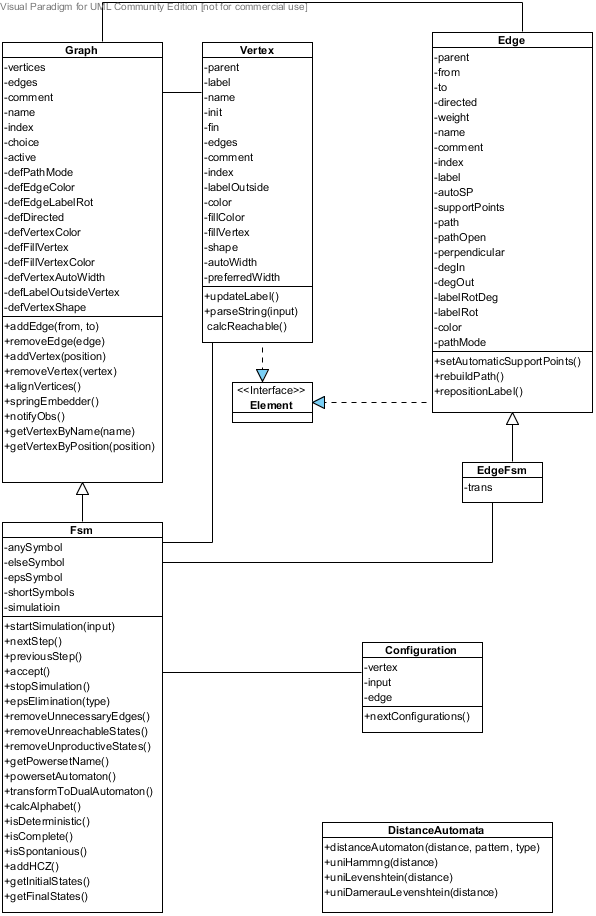
\includegraphics[width=\linewidth,height=\textheight,keepaspectratio]{pic/fsm}%
\caption{Klassendiagramm funktionale Klassen mit den wichtigsten Attributen und Methoden}%
\end{figure}
Die Hauptklasse ist die Klasse Graph, welche einen grundlegende Eigenschaften eines Graphen implementiert und die Knoten und Kanten hält.

Die Klasse Fsm erweitert die Klasse Graph um automatenspezifische Aspekte, das beinhaltet den Austausch der Kanten gegen eine für Automaten erweiterte Version, Methoden zur Simulation von Eingaben und die Algorithmen auf Automaten.

Knoten werden durch die Klasse Vertex repräsentiert, Kanten durch die Klasse Edge, bzw. EdgeFsm, welche die Kanten von Graphen um Übergänge erweitert. Diese Klassen implementieren das leere Interface Element, damit z.B. für eine Auswahl beide Klassen gleichartig gespeichert werden können.

Für die Simulation wird die Klasse Configuration benutzt. Sie repräsentiert einen Berechnungsschritt während der Simulation, also den aktuellen Zustand mit der Rest\-eingabe. Außerdem enthält die Klasse eine Funktion um eine Menge von Folgekonfigurationen zu berechnen.

Die Klasse DistanceAutomata enthält ausschließlich statische Methoden zur Erzeugung verschiedener Abstandsautomaten (universell und speziell).

\subsection{GUI-Klassen}
\begin{figure}[htbp]
\centering
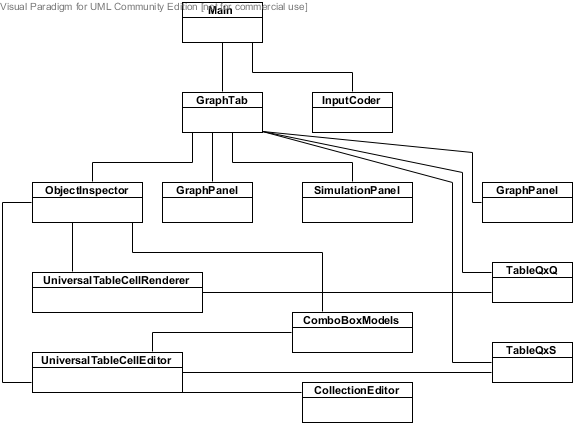
\includegraphics[width=\linewidth,height=\textheight,keepaspectratio]{pic/gui}%
\caption{Klassendiagramm GUI-Klassen ohne Attribute und Methoden}%
\end{figure}
Die Hauptklasse ist die Klasse Main. Sie ist ausführbar und erstellt ein JFrame mit einer Menüleiste und einer JTabbedPane. Hierin werden beliebig viele Automaten-/Grapheneinheiten repräsentiert durch die Klasse GraphTab. Hierin sind der Objektinspektor, die graphische Visualisierung, QxQ- und QxS-Tabelle und die Simulationssteuerung mit den entsprechenden Klassen Objectinspector, GraphPanel, TableQxQ, TableQxS und SimulationPanel angeordnet. Alle Tabellen (also QxQ, QxS und Objektinspektor) benutzen als Renderer zur Darstellung den UniversalTableCellRenderer und als Editor den UniversalTableCellEditor. Die Modelle, die den Tabellen die Daten liefern, sind Unterklassen der entsprechenden Komponente.

Die Klasse ComboBoxModels enthält Modelle und Renderer für ComboBoxen (mit Knoten oder mit Elementen).

Die Klasse CollectionEditor wird von dem UniversalCellEditor benutzt und zeigt ein Fenster zur Bearbeitung von Listen, Sets und Maps.

InputCoder ist ein Fenster, welches dazu da ist, die Eingabe für universelle Abstandsautomaten zu kodieren.

\section{parseString}
Bei den Beschriftungen von Knoten und Kanten ist Hoch- und Tiefstellen von Text möglich. Dafür sind zwei Implementierungen denkbar. Eine Möglichkeit wären Attributed Strings. Im folgenden Beispiel sind die Zahlen 5-7 hochgestellt.
\begin{lstlisting}
AttributedString as1 = new AttributedString("1234567890");
as1.addAttribute(TextAttribute.SUPERSCRIPT, TextAttribute.SUPERSCRIPT_SUPER, 5, 7);
g2d.drawString(as1.getIterator(), 15, 60);
\end{lstlisting}

Die Alternative beruht darauf, dass (fast) alle Swing-Komponenten HTML darstellen können. Das folgende Beispiel stellt ebenfalls die Zahlen 5-7 hoch. 
\begin{lstlisting}
label1.setText("<html>1234<sup>567</sup>890</html>");
\end{lstlisting}

Umgesetzt ist die zweite Methode. Beim setzten von Beschriftungen wird der String nach den formatierenden Symbolen (\_, \^\  und \textbackslash) gesucht und dann in entsprechenden HTML-Code umgesetzt. Dabei ist die Reihenfolge der Auswertung wichtig.
\begin{lstlisting}
		public static String parseString(String s) {
        StringBuilder t = new StringBuilder();
        Stack<String> open = new Stack<String>();
        boolean esc = false;
        boolean ins = false;
        boolean html = false;
        for (int i = 0; i < s.length(); i++) {
            final char c = s.charAt(i);
            if (esc) {
                t.append(c);
                esc = false;
                if (ins) {
                    t.append(open.pop());
                    ins = false;
                }
            } else if (c == '\\') {
                esc = true;
            } else if (ins && c != '{') {
                t.append(c).append(open.pop());
                ins = false;
            } else if (c == '_') {
                t.append("<sub>");
                open.add("</sub>");
                ins = true;
                html = true;
            } else if (c == '^') {
                t.append("<sup>");
                open.add("</sup>");
                ins = true;
                html = true;
            } else if (c == '{') {
                if (!ins) {
                    t.append(c);
                } else {
                    ins = false;
                }
            } else if (c == '}') {
                if (open.isEmpty()) {
                    t.append(c);
                } else {
                    t.append(open.pop());
                }
            } else {
                t.append(c);
            }
        }
        while (open.size() > 1) {
            t.append(open.pop());
        }
        if (ins) {
            if (open.pop().equals("</sub>")) {
                t.append('_');
            } else {
                t.append('^');
            }
        } else if (!open.isEmpty()) {
            t.append(open.pop());
        } else if (esc) {
            t.append('\\');
        }
        if (html) {
            t.append("</nobr></html>");
            t.insert(0, "<html><nobr>");
        }
        return t.toString();
    }
\end{lstlisting}
\section{Tabellen}
Tabellen in Java sind etwas gewöhnungsbedurftig, aber dafür recht mächtig. Es gibt drei Teile, über die man sich beim Bau einer Tabelle Gedanken machen muss.

Das erste ist das TableModel. Die wichtigen Methoden in dieser Klasse sind \lstinline[breaklines=true]{getValueAt(int rowIndex, int colIndex)} und für editierbare Tabellen \lstinline[breaklines=true]{isCellEditable(int rowIndex, int colIndex)} und \lstinline[breaklines=true]{setValueAt(Object value, int rowIndex, int columnIndex)}. Es gibt vorgefertigte einfache TableModels, die aber schnell an die Grenzen stoßen. Alle Table\-Mo\-dels (Objektinspektor, $Q \times Q$-Tabelle und $Q \times S$-Tabelle) sind überschrieben und geben in Abhängigkeit der Position direkt Daten des Graphen bzw. Automaten weiter bzw. schreiben diese Werte. Für Werte bei denen eine Referenz übergeben wurde und nur dieses Objekt bearbeitet und nicht überschrieben wurde (z.B. Listen) muss die setValueAt-Methode gar nichts unternehmen.

Der Renderer ist für die Darstellung verantwortlich. Der Defaultrenderer ist nur geeignet, wenn eine gesamte Spalte einen eindeutigen Typ hat. Dann kann er z.B. Boolean-Werte durch eine CheckBox darstellen. Objects werden einfach durch ihre Stringrepräsentation dargestellt. Alle Tabellen benutzen den UniversalTableCellRenderer, welcher die Methode \lstinline{public Component getTableCellRendererComponent(JTable table, Object value, boolean isSelected, boolean hasFocus, int row, int column)} überschreibt. In Abhängigkeit des Types von value (Test mit instanceof) wird eine geeignete Darstellung in einem JLabel erstellt und zurückgegeben.

Der Editor übernimmt die Bearbeitung der Werte. Zum einen muss die Methode \lstinline{public Component getTableCellEditorComponent(JTable table, Object value, boolean isSelected, int rowIndex, int colIndex)} überschrieben werden, welche -- wie beim Renderer -- abhängig vom Typ von value eine geeignete Komponente zur Bearbeitung des Wertes zurückliefert. Als zweites muss die Methode \lstinline{public Object getCellEditorValue()}, welche nach dem Beenden des Editierens aufgerufen wird und den neuen Wert an das TableModel zurück gibt, überschrieben werden. Dafür wird beim Wählen der Komponente diese gespeichert, damit dann daraus der Wert (mit dem richtigen Typ) zurückgegeben werden kann.

Ein Schwierigkeit bei der Implementierung war, dass das Beenden des Editierens einer Zelle nur durch explizite Aufforderung durch den Benutzer geschieht, also durch Auswahl einer anderen Zelle mit der Maus oder Bestätigen durch Enter oder Tab. Zum einen werden dadurch die neuen Werte erst spät übernommen, zum anderen kann es zu Problemen kommen, wenn sich während des Editierens der Inhalt der Zelle ändert, oder gar der Typ (z.B. wenn beim Objektinspektor ein anderer Elementtyp (Graph, Knoten, Kante) ausgewählt wird). Es soll eine Möglichkeit geben mit \lstinline{table.putClientProperty("terminateEditOnFocusLost", Boolean.TRUE);} das Editieren automatisch zu stoppen, aber das hat nicht funktioniert. Es funktioniert ebenfalls nicht, das Editieren zu Stoppen, wenn die Tabelle den Focus verliert, da die Tabelle den Focus auch nicht hat, wenn der Editor in der Tabelle ihn hat. Also muss jeder Editor einen FocusListener bekommen, in dem das Editieren bei FocusLost explizit gestoppt werden kann. Dabei ist zu beachten, dass z.B. JSpinner keinen Focus haben, sondern nur das TextFeld des Editors des Spinners, außerdem sollte dem TextFeld Focus gegeben werden, wenn direkt ein Button des Spinners benutzt wird. Weiterhin ist darauf zu achten, nicht bei jedem Focus-Verlust das Editieren zu beenden, denn wenn eine andere Zelle ausgewählt wird, wird das Editieren erst gestoppt und der nächste Editor erhält den Focus danach, d.h. es würde das Editieren sofort nocheinmal gestoppt werden. Ähnliches gilt, wenn der Editor aus mehreren Komponenten besteht (z.B. Punkte mit zwei Spinners). Die Probleme wurden gelöst, indem alle Editorkomponenten, die einen Focus erhalten können, in einer Liste gespeichert werden und beim FocusLost getestet wird, ob die neue Komponente mit dem Focus nicht in dieser Liste ist.

Weiterhin ist zu beachten, dass beim Stoppen des Editierens nicht automatisch die neuen Werte beim JSpinner gesetzt werden, es sollte also vor dem Abfragen der Werte ein \lstinline{((JSpinner.DefaultEditor) spinner.getEditor()).commitEdit()} aufgerufen werden. Bei Werten die über ein eigenes Fenster (Collection-Editor, Color) und bei Boolean-Werten sollte das Editieren automatisch sofort nach dem Zurückgeben der Komponente gestoppt werden, damit die Änderungen übernommen werden können. Das funktioniert, indem unmittelbar nach der Auswahl der Komponente, der stopEditing-Befehl in die Java-EventQueue eingetragen wird:
\begin{lstlisting}
java.awt.EventQueue.invokeLater(new Runnable() {
	@Override
	public void run() {
		stopCellEditing();
	}
});
\end{lstlisting}
Eine ComboBox sollte über einen ActionListener nach der Auswahl eines Wertes das Editieren beenden.\\
Außerdem wird für alle textuellen Editoren ein Timer gestartet, der nach 3 Sekunden ohne Eingabe das Editiern automatisch beendet (durch Key- und MouseListener wird dieser Timer bei beliebiger Interaktion neu gestartet).

\begin{table}
\begin{sloppypar}\noindent \begin{longtable}{p{(\textwidth-12\tabcolsep-12\fboxrule)/6}|p{(\textwidth-12\tabcolsep-12\fboxrule)/6+3pt}|p{(\textwidth-12\tabcolsep-12\fboxrule)/6-3pt}|p{(\textwidth-12\tabcolsep-12\fboxrule)/6}|p{(\textwidth-12\tabcolsep-12\fboxrule)/6}|p{(\textwidth-12\tabcolsep-12\fboxrule)/6}}
 \textbf{Typ}&\textbf{Werte}&\textbf{Renderer}&\textbf{Editor}&\textbf{Stop Editing}&\textbf{Listener}\\
 \hline\hline
 \endhead
String & Name, Kommentar & String & JTextField & Focus,\newline Timer & Focus,\newline Key, Mouse \\ \hline
Character & Automaten-Symbole & toString & JTextField mit DocumentFilter & Focus,\newline Timer & Focus, Key, Mouse \\\hline
Color & Farben & Label-Farbe, String, RGB-Wert & JColor\-Chooser & instantan & - \\\hline
Boolean & Initial, Final, Füllen, autom. Breite usw. & Haken/\newline Kreuz & JLabel & instantan & - \\\hline
Integer & Index, Breite, Höhe & toString & JSpinner & Focus,\newline Timer & (Focus,\newline Key,\newline Mouse,)\newline Change \\\hline
Double & Winkel, Gewicht & toString & JSpinner & Focus,\newline Timer & (Focus, Key,\newline Mouse,)\newline Change \\\hline
Point & Positionen & int, int & 2 JSpinner & Focus,\newline Timer & je (Focus, Key,\newline Mouse,)\newline Change \\\hline
Shape & Form & enum (String) & JCombo\-Box & Focus,\newline Auswahl & Focus,\newline Action \\\hline
PathMode & Ecken abrunden & enum (String) & JCombo\-Box & Focus,\newline Auswahl & Focus,\newline Action \\\hline
Vertex & Start, Ziel & getName() & JCombo\-Box & Focus,\newline Auswahl & Focus,\newline Action \\\hline
List & Hilfspunkte, QxS-Eintrag & zeilenweise & Collection\-Editor & instantan & - \\\hline
Set & Übergänge & zeilenweise & Collection\-Editor & instantan & - \\\hline
Map & Symbol\-abkürzungen & zeilenweise \newline Key $=>$ Val & Collection\-Editor & instantan & - \\\hline
\end{longtable}\end{sloppypar}
\caption{Übersicht über Typen und dazugehörige Editoren}
\end{table}
\section{Shapes}
Für die graphische Repräsentation der Knoten und Kanten werden Klassen, die das Interface Shape implementieren, benutzt. Knoten können beliebige RectangularShape annehmen; Arc2D, Ellipse2D, Rectangle2D und RoundRectangle2D werden von Java mitgeliefert. Bis auf Arc2D können diese Formen auch als Knotenform im Objektinspektor ausgewählt werden. Es wäre ohne weiteres möglich, eine Klasse zu schreiben, die RectangularShape implementiert und diese dann als Knotenform zu benutzen. Die Shape-Klassen lassen sich dann sehr leicht auf den graphischen Kontext eines Panels zeichnen. Mit der contains-Methode lässt sich überprüfen, ob z.B. ein Mausklick innerhalb eines Shapes gemacht wurde.

Kanten werden als Path2D repräsentiert. Dieser setzt sich aus Abschnitten von geraden Linien, quadratischen oder kubischen Bezierkurven zusammensetzen. Der Pfad wird vom Startknoten zum Zielknoten über die Hilfspunkte berechnet. Berechnung von Start und Zielpunkt erfordert etwas Rechnerei, weil es nicht ausreicht, vom Zentrum oder Rand der BoundingBox die Linie zu zeichnen, dadurch würde ein Teil der Linie innerhalb des Knotens liegen (was zum einen bei Transparenz ein Problem ist, zum anderen den Pfeil verschwinden lässt) oder die Linie in der Luft schwebt. Zunächst wird die Richtung bestimmt als Vektor zwischen Start bzw. Ziel und wenn vorhanden nächster Hilfspunkt oder Ziel bzw. Start berechnet. An diesem Vektor wird dann so lange \glqq entlang gelaufen\grqq, bis man gerade innerhalb des Knotens bzw. gerade außerhalb des Knotens ist (Überprüfung mit contains()).

Ohne Abrunden von Ecken wird einfach eine Linie von Hilfspunkt zu Hilfspunkt gezeichnet. Mit Abrundung werden Bezierkurven von dem Mittelpunkt der Verbindung letzter Hilfspunkt (bzw. Start) zum nächsten Hilfspunkt (bzw. Ziel) mit dem aktuellen Hilfspunkt als Stützpunkt gezeichnet. Bei starker Abrundung wird eine quadratische Bezierkurve benutzt. Bei leichter Abrundung wird eine kubische Bezierkurve mit dem aktuellen Hilfspunkt für beide Stützpunkte benutzt, wodurch der Hilfspunkt stärker gewichtet wird. Die fehlenden Enden werden durch einfache Linien ergänzt.

Die Auswahl der Pfade erfolgt mit der intersect-Methode und einem um den gewünschten Punkt gelegtem Kreis. Dabei ist es ärgerlich, dass Java den Pfad automatisch schließt -- grundsätzlich durch eine direkte Verbindung von Start und Ziel. Das ist unproblematisch ohne Hilfspunkte, aber mit Hilfspunkten entstehen dadurch unerwünschte Formen mit einem echten Flächeninhalt. Um dies zu umgehen, muss der Pfad nocheinmal komplett rückwärts berechnet werden. Es werden also zwei Pfade für eine Kante gehalten, einmal der einfache zum Zeichnen und ein weiterer geschlossener zur Überprüfung eines Schnittes. Die Punkte des Pfeiles müssen extra berechnet werden unter Berücksichtigung der entsprechenden Winkel.

Die Beschriftungen sind in JLabels gespeichert. Es hat sich herausgestellt, dass man es vermeiden sollte, die Labels dem Container hinzuzufügen, da dadurch durchgehend repaints aufgerufen wurden. Stattdessen sollte man die Labels mit der paint-Methode in den graphischen Kontext des Panels zeichnen. Das bedeutet, dass man keine Mouse-Listener auf den Labels verwenden kann, sondern in dem MouseListener des Panels über contains überprüft werden muss, ob der Mausklick im Label war. Gleichzeitig wird es dadurch sehr einfach, das Label zu drehen, indem man vor dem Zeichnen den graphischen Kontext dreht. Diese Drehung muss auch bei der contains-Überprüfung beachtet werden.
\section{Defaultwerte}
Zunächst waren die Default-Werte als statische Klassenattribute direkt in der Kante bzw. dem Knoten gespeichert. Das hat den großen Nachteil, dass bei mehreren geöffneten Automaten bzw. Graphen die Defaultwerte global für alle gelten. Außerdem werden dadurch die Defaultwerte nicht mitgespeichert.

Die Alternative war, die Defaultwerte im Graphen (Automaten) zu speichern und in den Knoten-/Kantenobjekten das Elternelement zu speichern, damit auf diese Werte zugegriffen werden kann.

Ein weiterer Aspekt war, dass zunächst ein boolean-Attribut inherit benutzt wurde, welches angegeben hat, ob die Kante bzw. der Knoten die Standardeinstellungen erben soll. In diesem Fall wurde direkt der Standardwert im Getter zurückgegeben. Bei der Änderung eines solchen Wertes wurde auf inherit auf false gesetzt. Diese Art des inherit-Flags hatte den Vorteil, dass, wenn der Standard-Wert geändert wurde, dieser sofort automatisch von den Knoten bzw. Kanten übernommen wurde. Auf der anderen Seite entstanden dadurch unschöne Effekte, dass sich  mit dem Ändern des inherit-Flags mehr Eigenschaften änderten, als eigentlich der Fall sein sollte. Deshalb wurde das Flag entfernt und stattdessen gibt es eine Methode, um die Werte zurück auf die Defaultwerte zu setzen. Nun werden Änderungen der Defaultwerte selbst nicht rückwirkend übernommen und gelten nur für neue Kanten und Knoten. Es wäre aber denkbar, dafür eine Option einzubauen, die dafür sorgt, dass der Defaultwert auch bei bereits vorhandenen Elementen gesetzt wird.
\section{Graph/Fsm-Erweiterung}
Da die Automaten eine graphische Darstellung unterstützen sollen, können Automaten als Graphen mit zusätzlichen Eigenschaften, die speziell für Automaten benötigt werden, betrachtet werden. Es bietet sich daher an, zunächst eine Klasse Graph zu erstellen, die alle Informationen für eine graphische Darstellung mit Knoten und Kanten enthält und diese dann um die zusätzlichen Funktionen zu erweitern. Das bietet die Möglichkeit, im Programm auch Graphen ohne Automateneigenschaften zu konstruieren. Lediglich zwei Eigenschaften von Graphen haben für Automaten keine Bedeutung, nämlich Kantengewichte, welche aber nicht stören, und die Möglichkeit ungerichtete Kanten zu benutzen. Das wird im Automaten durch ein Überschreiben der Setter-Methode für diesen Wert erreicht.

Beim Erweitern des Graphen müssten auch die Klassen Edge und Vertex erweitert werden, da die wesentlichen Eigenschaften der Automaten in diesen Klassen liegen. Kanten benötigen zusätzlich die Übergangsrelation und Knoten die Eigenschaften Start- bzw. Finalzustand. (Für die Potenzmengenkonstruktion haben die Knoten auch noch Felder und Methoden zur Berechnung der erreichbaren Zustände). Die Klasse Edge wurde auch tatsächlich mit EdgeFsm um die Übergangsrelation erweitert. Nachteil davon ist, dass auch z.B. Methoden zum Hinzufügen im Automaten durch die andere Klasse überschrieben werden müssen. Auch erfordert dies öfters Casts, wenn zunächst nur die allgemeine Kantenklasse vorliegt und die Automateneigenschaften benötigt werden. Wegen dieser Unbequemlichkeiten wurde bei den Knoten zunächst darauf verzichtet, diese zu erweitern, sondern die benötigten Felder und Methoden liegen in der allgemeinen Knotenklasse Vertex, da diese Graphen nicht stören. Der Sauberkeit halber sollte eine Trennung in Vertex- und VertexFsm-Klasse nachgeholt werden.
\section{Simulation}
Zunächst war die Simulation so implementiert, dass in einer Liste die aktiven Zustände (und zur Darstellung aktive Kanten) gespeichert wurden und global der Resteingabe-String. Bei der Berechnung des nächsten Schrittes wurde von jedem aktiven Zustand die Erreichbarkeit mit der Resteingabe überprüft und die Resteingabe entsprechend angepasst. Die neuen aktiven Elemente waren dann die benutzen Kanten mit ihren Zielzuständen. Spontan erreichbare Zustände wurden nach jedem Berechnungsschritt hinzugefügt. Das funktioniert einfach und gut, solange die Blocklänge konstant ist und keine spezielle Berechnung nachvollzogen werden soll, denn dafür werden mehr Informationen gebraucht, bzw. unterschiedliche Berechnungen können eine unterschiedliche Resteingabe haben.

Jetzt hält die Simulation eine Liste von Berechnungen, was einer Liste einer Liste von Konfigurationen entspricht, wobei eine Konfiguration ein aktiver Zustand mit der dazugehörigen Resteingabe ist. Eine Konfiguration wird durch die Klasse Configuration repräsentiert. Zusätzlich kann zur Visualisierung die aktive Kante gespeichert werden. Die Klasse Configuration bietet eine Methode, um eine Liste von Folgekonfiguration zu berechnen. Spontane Übergänge erfolgen nun wie andere Übergänge auch in einem eigenen Simulaitonsschritt. Die Liste der aktiven Elemente wird weiterhin für die Visualisierung genutzt und muss entsprechend nach einem Berechnungsschritt aus der Konfiguration berechnet werden.

Bei der Berechnung der Folgekonfigurationen wird jeder von dem Zustand der Konfiguration aus mögliche Übergang mit dem Beginn der Resteingabe gleicher Länge verglichen. Dabei gibt es einige Besonderheiten. Any-Übergänge funktionieren immer. Spontane Übergänge auch, verbrauchen aber keinen Buchstaben und müssen für Else-Übergänge gezählt werden. Else-Übergänge müssen zunächst gemerkt werden, diese werden nur den Übergängen hinzugefügt, wenn nur spontane gemacht wurden (deshalb müssen sie gezählt werden). Tritt keiner dieser Sonderfälle auf, wird der Block (auch Länge 1) zeichenweise verglichen. Dabei müssen die Abkürzungssymbole umgesetzt werden.

Der Start der Simulation erfolgt mit der Methode startSimulation(String input). Beim Start der Simulation werden Konfigurationen mit der vollen Eingaben für jeden Startzustand in die Liste eingetragen. Der nächste Simulationsschritt wird mit der Methode nextStep() berechnet. Dabei wird für jede letzte Konfiguration der Berechnung in der Liste der Berechnungen die Folgekonfigurationen berechnet. Die alte Berechnung wird aus der Liste entfernt und für jede Folgekonfiguration wird die alte Berechnung konkateniert mit der entsprechenden Folgekonfiguration wieder hinzugefügt. Dabei muss explizit der Fall ausgeschlossen werden, dass ein spontaner Kreis geschlossen wird, was nicht zur Erkennung der Sprache beiträgt, aber unendlich lange Berechnungen produziert. Dafür wird für jede Konfiguration mit gleichem Input überprüft, ob bereits eine Konfiguration mit dem gleichen Zustand existiert.
\section{Algorithmen}
\subsection{Automaten optimieren}
Zu dieser Kategorie zählen Entfernen von unproduktiven Zuständen, Entfernen von unerreichbaren Zuständen, Entfernen unnötiger und zusammenfassen mehrfacher Kanten und das Hinzufügen eines Hotel-California-Zustanden. All dies sind wenig komplexe Algorithmen.

Für das Auffinden von unerreichbaren Zuständen wird von den Startzuständen aus eine Breitensuche durchgeführt, für das Auffinden von unproduktiven Zuständen wird dies im dualen Automaten gemacht. Dabei werden die erreichbaren Zustände durch die Startzustände initialisiert. Zu diesen Zuständen wird sich gemerkt, ob sie schon verarbeitet wurden. Für alle erreichbaren, aber nicht verarbeiteten Zustände, werden die Nachbaren zu den erreichbaren Zuständen hinzugefügt, anschließend wird dieser Zuständ als verarbeitet markiert. Wenn keine Änderungen mehr auftreten, also alle erreichbaren Zustände verarbeitet wurden, sind alle erreichbaren Zustände gefunden und die übrigen können entfernt werden.

Für die Optimierung der Kanten wird durch alle Kanten iteriert. Ist die Übergangsmenge leer, wird die Kante entfernt. Andernfalls wird überprüft, ob bereits eine Kante mit den selben Start- und Zielzuständen gefunden wurde. Ist dies der Fall, werden alle Übergänge den Übergängen der anderen Kante hinzugefügt und diese Kante entfernt.

Das Hinzufügen eines HCZ kann intelligent oder nicht intelligent geschehen. Bei der nicht intelligenten Form wird einfach ein Zustand, welcher weder Start- noch Endzustand ist, ergänzt und von jedem Zustand aus wird ein Else-Übergang zu diesen Zustand hinzugefügt. Bei der intelligenten Version muss zunächst das Alphabet berechnet werden. Dann werden nur dann Übergänge mit den verbliebenden Zeichen hinzugefügt, wenn der Zustand lokal nicht vollständig ist. Wie bei der globalen Vollständigkeit, ist die Überprüfung auf lokale Vollständigkeit bei variabler Blocklänge sehr schwierig. Außerdem könnte überprüft werden, ob bereits ein HCZ existiert und dieser benutzt werden. Die intelligente Variante ist noch nicht implementiert.
\subsection{Dualer Automat}
Die Berechnung des dualen Automaten ist sehr einfach. Zunächst wird durch alle Zustände iteriert. Ist ein Zustand Startzustand, wird er Endzustand und umgekehrt. Anschließend wird durch alle Kanten iteriert und Start- mit Zielknoten vertauscht.
\subsection{Epsilon-Elimination}
Die Elimination spontaner Übergänge kann durch Absorbtion von links, rechts oder beidseitig erfolgen. Bei der Absorbtion von links werden erst spontane Übergänge gemacht und dann der normale Übergang angehängt, von rechts erst normaler Übergang und dann spontane Übergänge und beidseitig werden vorher und nacher spontane Übergänge gemacht.

Es wird also von jedem Zustand n aus bei nicht rechts die Epsilon-Erreichbarkeit berechnet, sonst ist nur n erreichbar. Nun wird vom Zustand n für jede Kante e eine Kante mit dem Übergang von n zum Zielknoten von e hinzugefügt. Bei nicht links außerdem zu den vom Zielknoten von e durch spontane Übergänge erreichbaren Zuständen. Es spielt keine Rolle, ob dabei spontane Kanten kopiert wurden. Die neuen Kanten müssen gespeichert werden, da die neuen Kanten im vorigen Schritt nicht benutzt werden dürfen. Erst am Ende werden die spontanen Übergänge selbst entfernt.
\subsection{Potenzmengenkonstruktion}
Durch die Sonderfunktionen bei der Berechnung ist die Potenzmengenkonstruktion sehr aufwändig.

Zunächst muss von jedem Knoten die Erreichbarkeit (ohne spontane Übergänge) berechnet werden. Diese wird in einer Map gespeichert, die von Übergangslabeln auf eine Menge von Zuständen abbildet. Dabei wird jeder mögliche Übergang betrachtet, wobei Any und Else-Übergänge nicht gesondert betrachtet werden und spontane Übergänge übersprungen werden. Der durch den Übergang erreichbare Zustand sei n. Existiert dieser Übergang in der Map, wird n der dazugehörigen Zustandsmenge hinzugefügt. Existiert er nicht, muss überprüft werden, ob es eine Überschneidung von diesem Übergang mit einem Übergang in der Map gibt, was durch die abkürzenden Symbole vorkommen kann. Gibt es eine Überschneidung, müssen dieser Eintrag entfernt und bis zu drei neue Einträge hinzugefügt werden: ein Eintrag, mit dem Übergangslabel, das übrig bleibt, wenn man die Überschneidung von dem ursprünglichen Übergang abzieht, und der ursprünglichen Zustandsmenge, ein Eintrag mit der Überschneidung und der ursprünglichen Zustandsmenge erweitert um n und ein Eintrag mit dem Übergangslabel, das übrig bleibt, wenn man die Überschneidung vom aktuellen Übergang abzieht, und n. Gibt es keine Überschneidung wird ein neuer Eintrag mit dem aktuellen Übergang und n angelegt.

%intersection berechnen
Um die Überschneidung zu berechnen, werden beide Übergänge zeichenweise verglichen. Stimmen die Zeichen überein (auch bei Symbolabkürzungen), ist dies ein Teil der (potentiellen) Überschneidung. Ist dies nicht der Fall, müssen beide Zeichen auf Symbolabkürzungen überprüft und ggf. miteinander verglichen werden. Finden sich dabei keine gleichen Zeichen, gibt es keine Überschneidung. Beim Vergleich ist es möglich, dass mehrere Zeichen gleich sind und so mehrere Überschneidungen entstehen. %TODO gedanken über präfixe, ich glaube das stimmt so nicht, wie es gerade ist.

%remaining berechnen
Um die Reste zu berechnen, wird für jedes Symbol des ersten Strings die entsprechende Menge von Zeichen angelegt, wobei die Zeichen des zweiten Strings jeweils abgezogen werden. Jedes in den den Mengen verbliebende Zeichen wird dann einmal an entsprechender Stelle im ersten Originalstring eingesetzt und der Menge der Reste hinzugefügt.

Bei der eigentlichen Potenzmengenkonstruktion wird mit dem Metazustand, der aus der Menge der Startzustände besteht gestartet. Für diesen und jeden weiteren entstandenen Metazustand wird folgendes getan. Die Übergänge aller Zustände der Zustandsmenge des Metazustandes werden zusammengefasst und zwar auf die gleiche Art wie bei der Berechnung der Erreichbarkeit von einem Knoten aus. Bei dieser Gelegenheit werden gleich leere Else-Übergänge entfernt, also wenn es zu dem Else-Übergang noch ein Any-Übergang beim gleichen Knoten gibt. Anschließend müssen Any- und Else-Übergänge gesondert behandelt werden. Die Zustände, die über das Any-Symbol erreichbar sind, müssen jedem Übergang hinzugefügt werden. Die Zustände, die über das Else-Symbol erreichbar sind, müssen jedem Übergang der anderen Knoten hinzugefügt werden. Any-Symbole werden anschließend zu Else-Symbolen. Nun werden entsprechend der berechneten Übergänge Kanten und - sofern sie noch nicht existieren - neue Metazustände angelegt.
\begin{figure}[!htbp]
\centering
\subfloat[Any: Der zusammengesetzte Automat links wird zum Potenzmengenautomat rechts. Der Else-Übergang zu q$_6$ entfällt. Die Ziele der Any-Übergänge müssen sowohl den Zielen von 1 also auch den Zielen von 0 hinzugefügt werden. Damit kann der Any-Übergang dann zum Else-Übergang werden, um Determinismus zu gewährleisten.]{
\includegraphics[scale=0.7]{pic/automata/beispielPMAany}}%
\hspace{0.1cm}
\subfloat[Else: Der zusammengesetzte Automat links wird zum Potenzmengenautomat rechts. Die Else-Übergänge werden jeweils nur den Übergängszielen der Übergangslabels des anderen Teilautomaten hinzugefügt.]{
\includegraphics[scale=0.7]{pic/automata/beispielPMAelse}}%
\caption{Beispiele Potenzmengenkonstruktion Any und Else-Übergänge}%
\end{figure}

\subsection{Automateneigenschaften}
Vollständigkeit: Um die Vollständigkeit zu überprüfen, muss zunächst das Alphabet berechnet werden. Für variable Blockgrößen ist schwer feststellbar, ob der Automat vollständig ist. Bei konstanter Blockgröße größer als 1, ist zu entscheiden, ob ein Automat als vollständig gelten kann, da in dem Fall die Eingabe ein Vielfaches der Blockgröße sein muss, damit der letzte Schritt funktionieren kann. Grundidee ist für Automaten ohne Blöcke zu kontrollieren, ob für jedes Zeichen des Alphabetes ein Übergang existiert.\\
\textit{Hinweis: Die Funktion ist für Blöcke nicht vollständig implementiert.}

Determinismus: Beachte die hier benutzte Definition von Determinismus (\ref{Determinismus}). Bei der Überprüfung, ob der Automat deterministisch ist, muss überprüft werden, ob von einem Zustand bzw. der Epsilon-Erreichbarkeit ein Übergäng Präfix eines anderen ist (also evt. auch gleich ist).\\
\textit{Hinweis: Die Funktion ist für Blöcke nicht vollständig implementiert.}

Alphabet: Die Berechnung des Alphabetes erfolgt, indem jeder Übergang betrachtet wird und eine Liste der benutzten Zeichen erstellt wird. Blöcke werden dabei in ihre einzelnen Zeichen zerlegt. Any-, Else- und spontane Symbole werden dabei nicht berücksichtigt. Symbolabkürzungen werden umgesetzt.

Spontanität: Die Überprüfung, ob der Automat spontane Symbole benutzt, erfolgt durch ein Durchsuchen sämtlicher Übergänge nach dem spontanen Symbol.

Initial- bzw Finalzustande: Für die Rückgabe der Initial- bzw Finalzustande werden alle Zustände durchlaufen und ein Zustand der Liste hinzugefügt, wenn er entsprechend Initial- oder Finalzustand ist.
%\subsection{Kleene-Algorithmus}
%\subsection{Minimierung}
\endinput

\chapter{Abstandsautomaten}\label{Abstandsautomaten}
Diese Kapitel beschreibt die theoretischen Ergebnisse in Bezug auf die Abstandsautomaten.
\section{Spezielle Abstandsautomaten}
Der Abstand oder die Distanz zwischen zwei Wörtern ist definiert als die minimale Anzahl an Operationen, die benötigt werden um ein Wort in das andere zu überführen. Welche Operationen dabei erlaubt sind, hängt von dem Abstand ab. Abstände sind Metriken auf dem Raum von Symbolsequenzen.
\subsection{Hamming-Abstand}
Beim Hamming-Abstand ist nur Substitution von Buchstaben erlaubt. Das bedeutet insbesondere, dass Muster und Vergleich die gleiche Länge haben müssen.

\textit{Bild}
Die unterste Zeile ist die Zeile ohne Fehler, jeweils eine Zeile höher bedeutet ein Fehler mehr. Die Anzahl der Zeilen entspricht also dem Abstand + 1. Mit jedem Buchstaben der Eingabe wandert man eine Spalte nach rechts. Ein waagerechter Else-Übergang bedeutet ein zum Muster passender Buchstabe, ein diagonaler ein nicht passender.
\subsection{Levenshtein-Abstand}
Der Levenshtein-Abstand erlaubt zusätzlich zur Substitution von Buchstaben auch Einfügungen und Löschungen von Buchstaben.
\textit{Bild}
Der Grundaufbau ist derselbe wie bei dem Hamming-Automaten. Es kommen lediglich zwei Übergängstypen hinzu. Die senkrechten Else-Übergänge bedeutet ein Einfügen eines Buchstabens, die diagonalen spontanen Übergänge das Löschen eines Buchstabens.

\subsection{Damerau-Levenshtein}
Der Damerau-Levenshtein-Abstand erlaubt zusätzlich zur Substitution, Einfügung und Löschung von Buchstaben Transposition benachbarter Buchstaben. In der Praxis ist dies relevant, da Vertauschen benachbarter Buchstaben ein typischer Tippfehler ist. Sowohl Substitution als auch Transposition könnte durch zwei Operationen (Einfügen und Löschen) erreicht werden. Jedoch führt dies zu einem anderen Abstand.
\section{Motivation universeller Automaten}
Anwendungsgebiete von Abstandsautomaten ist z.B. die Rechtschreibkorrektur, wobei ein Wort, dass nicht im Wörterbuch gefunden wird mit einem bestimmten Abstand auf jedes Wort im Wörterbuch getestet wird. Die akzeptierten Wörter bilden dann die Menge der Korrekturvorschläge. Andere Anwendungen wären z.B. alternative Suchvorschläge (\glqq Meinten Sie ...\grqq) oder bei fehlerbehafteter Datenübertragung.

Der Test des Abstandes muss oft sehr schnell gehen, da sehr viele Teste durchgeführt werden sollen. Während der Automat für Hamming deterministisch ist, gilt dies nicht für Levenshtein- und Damerau-Levenshtein-Automaten (Problem ist die Entscheidung welche Operation benutzt werden soll). Simulation von Nichtdeterminismus bedeutet einen deutlich größeren Aufwand. Auch das Umwandeln der NEAs in äquivalente DEAs durch Potenzmengenkonstruktion ist relativ aufwändig und die resultierenden Automaten wären sehr groß (Abhängig von der Länge des Musters).

Dadurch ist die Idee motiviert universelle Abstandsautomaten einzuführen. Dabei muss nur ein einziges mal (für einen festen Abstand) der Automat konstruiert werden (und ggf. deterministisch gemacht werden). Der Preis dafür ist eine nötige Kodierung der Eingabe.

Die Idee eines universellen Levenshteinautomaten wurd in Mihov und Schulz: Fast Approximate Search in Large Dictionaries, 2004 vorgestellt. Ziel dieser Arbeit ist es, die dort vorgestellte Form des Automaten zu untersuchen und Funktionsweise und Konstruktion zu erläutern. Außerdem sollen universelle Abstands-Automaten auch fuer den (einfacheren) Hamming-Abstand und den (komplizierteren) Damerau-Levenshtein-Abstand zu untersucht werden.
\section{Ergebnisse}
\subsection{Hamming-Abstand}
Ein universeller Abstandsautomat für den Hamming-Abstand ist durchaus möglich, aber überflüssig. Der Aufwand zu Kodierung der Aufgabe ist größer als die Berechnung des Abstandes selbst. Außdem ist der spezielle Hamming-Automat bereits deterministisch
\subsection{Levensheitn-Abstand}
Die Idee beim universellen Automaten für den Levenshtein-Abstand ist, dass in jedem Schritt die gleiche Entscheidung getroffen werden muss. Wird ein passender, ein löschender, ein einfügender oder ein substituierender Schritt gemacht. Die einzigen Vorinformationen die benötigt werden sind, wieviele Fehler wurden bereits gemacht und mit dem wievielten Buchstaben des Musters muss ich vergleichen, denn die Zahl der Berechnungsschritte lassen sich nicht eins zu eins auf die Buchstaben des Musters abbilden. Wurde ein Buchstabe gelöscht, muss ein Buchstabe weiter vorne im Muster abgeglichen werden. Wurde ein Buchstabe eingefügt, muss ein Buchstabe weiter hinten abgeglichen werden. Substitution und passende Übergänge ändern dies nicht. Die Anzahl der Fehler lassen sich leicht im Zustand kodieren. Allerdings muss in jedem Zustand der Vergleich zu jedem möglichen Musterbuchstaben (beschränkt durch den Abstand) zur Verfügung stehen. Welcher Vergleich betrachtet wird, wird wieder im Zustand kodiert.

Betrachtet man die erreichbaren Zustände nach n verarbeiteten Buchstaben der Eingabe im speziellen Automaten liefert das ein gleichschenkliges Dreick mit der Spitze unten (vgl. Bild). Dies sind die Zustände, die im universellen Automaten vorkommen. Damit für den Beginn und das Ende, wenn die Dreicke nicht mehr vollständig sind, keine gesonderte Behandlung erfolgen muss, werden einfach virtuelle Zustände an den fehlenden Stellen angenommen. Dies findet sich in der Kodierung wieder.

Die Kodierung muss also für jeden Berechnungsschritt einen Block liefern der Größe $2*k+1$ liefern, wobei $k$ der Abstand ist. Dieser Block wird in Mihov/Schulz charakteristischer Vektor genannt. Jedes Zeichen des charakteristischen Vektors ist entweder eine 0 oder eine 1, je nachdem ob der Buchstabe der Eingabe mit dem entsprechenden Buchstaben des Teils des Musters übereinstimmt. Da bei Beginn der Simulation kein Fehler gemacht wurde, ist zunächst der mittlere Buchstabe relevant, deshalb muss der erste Teil der Musters in der Mitte beginnen und die ersten k Symbole sind 0 (werden z.B. mit einem Buchstaben verglichen, der im Alphabet nicht vorkommt, vergleiche virtuelle Zustände im oben beschriebenen Dreieck). In jedem Schritt wird der Vergleichsblock um 1 nach links geshiftet und mit dem nächsten Buchstaben aus dem Muster aufgefüllt. Ist das Muster zu Ende, werden wie am Anfang Dummy-Buchstaben eingefügt. Es müssen so viele charakteristische Vektoren erzeugt werden, bis die Eingabe zu Ende ist und das letzte Zeichen des Musters an erster Stelle im Vergleichsblock ist. All diese charakteristischen Blöcke werden dann konkateniert und bilden die tatsächliche Eingabe zur Simulation.\\
Beispiel Eingabe Majah bei dem Muster Maya für den Abstand 2.\begin{longtable}{c|c||c}
Eingabesymbol & Vergleichsblock & kodierter Block/""charakteristischer Vektor \\ \hline \endhead
M & \$\$May & 00100 \\
a & \$Maya & 00101 \\ 
j & Maya\$ & 00000 \\
a & aya\$\$ & 10100 \\
h & ya\$\$\$ & 00000 \\
\$ & a\$\$\$\$ & 01111 \\
\end{longtable}

Sei die signifikaten Stelle eines Zustandes Stelle Mitte + Löschvorgänge - Einfügevorgänge. Unabhängig von der Fehleranzahl gibt es in jedem Zustand eine Schleife mit einer 1 an der signifikanten Stelle, die restlichen Stellen spielen keine Rolle (dürfen also 0 oder 1 sein). Diese Schleife repräsentiert der Fall, dass kein Fehler an dieser Stelle gemacht werden muss. Für den Fehlerfall gibt es drei Übergänge zu den erreichbaren Zuständen der nächsten Fehlerstufe. Für einen Einfügevorgang und einen Substitutionsvorgang hat der Übergang an der signifikanten Stelle eine 0, wobei die anderen Zeichen wieder keine Rolle spielen. Es ist ebenso möglich, an der Stelle auch eine 1 zu akzeptieren, in diesem Fall wird der Automat allerdings nicht minimal (und der Potenzmengenautomat wird auch größer). Der Löschvorgang hat die Besonderheit, dass der soeben verarbeitete Buchstabe anschließend noch verglichen werden muss. Dafür gibt es zwei Möglichkeiten. Zum einen kann der Übergang mit einer 0 an der signifikanten Stelle und einer 1 an der signifikanten Stelle + 1. Dies deckt jedoch nicht den Fall ab, dass mehrere Löschvorgänge hintereinander gemacht werden können. Dafür werden zusätzliche Kanten in die höheren Fehlerstufen benötigt mit 0 an der signifikaten Stelle des Startzustandes und einer 1 an der signifikanten Stelle des Zielzustandes. Die Alternative ist, diesen Übergang spontan zu machen, was aber bedeutet diesen Übergang auch bei einem fehlerlosen Übergang zu ermöglichen, wodurch -- wie oben -- ein nicht größerer Automat entsteht.

Der Startzustand ist der einzige Zustand in der fehlerfreien Stufe. Alle Zustände sind Endzustände. Die Erkennung des Endes der Eingabe wird durch die Kodierung des Wortes abgedeckt. Dieser NEA kann dann durch Potenzmengenkonstruktion in einen DEA umgewandelt werden.
\subsection{Damerau-Levenshtein}
Ausgegangen wird von dem universellen Levenshtein-Automaten aus dem letzten Abschnitt. Die Kodierung der Eingabe ist dieselbe.

Für jeden Zustand in allen Fehlerstufen außer der letzten, wird ein zusätzlicher Zwischenzustand benötigt. Dieser ist dadurch motivert, dass eine Transposition zwei Vergleiche benötigt, um erkannt zu werden. Der Tausch eines Zeichens von hinten nach vorne und umgekehrt ist äquivalent, es muss also nur ein Fall behandelt werden. Zu diesem Zwischenzustand geht also ein Übergang mit einer 0 an der signifikaten Stelle des Zustandes und einer 1 an der signifikaten Stelle + 1. Von diesem Zwischenzustand geht ein Übergang mit einer 1 an der signifikaten Stelle - 1 zu dem Zustand mit derselben signifikaten Stelle in der nächsten Fehlerstufe.

\textit{Das scheint noch nicht ganz auszureichen. bdac ist mit drei Tauschoperationen aus abcd erzeugbar, aber mit diesem Prinzip nicht erkennbar, weil zwei Komponenten von getauschten Paaren nocheinmal getauscht werden. Aber die Grundidee sollte richtig sein...}
\section{Vergleich zu Mihov/Schulz}
Die grundsätzliche Funktionsweise des hier vorgestellten Levenshteinautomaten ist die gleiche wie bei Mihov/Schulz. Es gibt jedoch ein paar unterschiede. Lihov/Schulz benutzt eine getrennte Nicht-Endzustand und Endzustandmenge, sie erweitern also am Ende die Dreiecke nicht um virtuelle Zustände. Entsprechend wird in der Kodierung, wenn das Muster zu Ende ist keie Dummy-Symbole eingefügt, sondern der charakteristische Vektor wird kürzer. Die Anzahl der charakteristischen Vektoren ist hier genau die Länge der Eingabe. Diese Vorgehen macht es allerdings nötig, den charakteristischen Vektor um eine Stelle zu erweiern. Diese Stelle wird benutzt, um zu überprüfen, ob das Ende der Eingabe erreicht ist, denn wenn der charakteristische Vektor nicht mehr vollständig ist, wird in die Endzustandsmenge gewechselt.

Das bedeutet, dass der Mohov/Schulz-Automat eine größere Zustandsmänge hat (mehr als die Hälfte kommt nochmal dazu) und eine andere Eingabewortlänge. Auf der einen Seite wird pro Vektor ein Zeichen mehr benötigt, auf der anderen Seite werden die Vektoren am Ende kürzer. Es kann außerdem sein, dass bei der hier vorgestellten Methode mehr charakteristische Vektoren berechnet werden müssen. Auf der anderen Seiten ist eine konstante Blockgröße vorteilhaft bei der Simulation. Große Abweichgungen (also größer als der Abstand) kann bereits bei der Kodierung abgefangen werden, da diese Wörter nicht akzeptiert werden können. Das gleicht den großen Unterschied der Eingabegrößen bei kurzer Eingabe zu einem langen Muster aus.

Außerdem wurde bei Mihov/Schulz direkt ein DEA konstruiert ohne den Zwischenschritt über den NEA. Dabei betrachten sie direkt eine optimierte Potenzmenge der Zustände in dem Dreieck, was genau den Zuständen entspricht, die die Potenzmengenkonstruktion bei den Übergängen mit geforderter 0 ergibt.

\textit{Es sollte wohl noch beschrieben werden, wie die Potenzmenge optimiert wird und wie die Übergänge bei Mihov/Schulz zustandkommen, was aber doof zu erklären ist und auch in dem Paper nicht wirklich erklärt wird.}

\chapter{Future Work}\label{FutureWork}
Das Projekt bietet viele Erweiterungsmöglichkeiten. Einige seien hier vorgestellt.

Zunächst wäre es sehr nützlich, (mindestens) einen funktionierenden Algorithmus zum Graphzeichnen zu haben. Gerade die bei der Potenzmengenkonstruktion entstehenden Automaten haben meist ein sehr schlechtes Layout.

Als Erweiterung für den Bedienkomfort wären Aspekte wie Zoom, um z.B. schnell einen Überblick über große Graphen zu bekommen, Mehrfachauswahl, um gannze Teile des Graphen zu verändern oder verschieben und eine Rückgängig-Option. Interessant wäre eine Möglichkeit Graphen nach TeX zu exportieren, wahlweise als TikZ-Bild oder als pstricks-Bild. Eine sehr große Erweiterung wäre z.B. die Erweiterung von Graphen auf eine dritte Dimension. Damit ließen sich komplexe Graphen teilweise deutlich besser anordnen. Zusätzliche graphische Elemente dürfte sich zwar weitgehend durch Knoten simulieren lassen, aber eine bessere Unterstützung wäre durchaus vorstellbar. Insbesondere im Zusammenhang mit der Mehrfachauswahl wäre eine Methode zum Gruppieren von Elementen gut.

So wie die Automaten lediglich eine Erweiterung der Graphen sind, könnte man die Automaten recht leicht erweitern um einen Stack, um auch Kellerautomaten zu betrachten und simulieren. Unterstützung für Turingmaschinen wäre vermutlich etwas aufwändiger, aber das Programm wäre eine geeignete Grundlage.

Weitere Algorithmen, die zu implementieren sind, wären der Kleene-Algorithmus zur Identifikation der Sprache durch reguläre Ausdrücke und die Minimierung von DEAs und evt. auch die aufwändigere Minimierung von NEAs. Aufwändig, aber interessant, wäre eine Simulation aller Algorithmen, was den Wert als didaktisches Begleitwerkzeug zur Theoretischen Informatik erheblich steigern würde.

Weiterhin könnte man das Programm als Grundlage für graphentheoretische Probleme benutzen. Eine Vielzahl von Algorithmen ließen sich implementieren, wie z.B. Breiten- und Tiefensuche, Dijkstra, Kruskal, Bellmann-Moore-Ford usw. Auch eine Untersuchung des Graphen auf besondere Eigenschaften wie Baumstruktur, Zusammenhang oder Planarität wären denkbar.


%%% Anhang
\bibliography{lit} %%% obligatorisch
\printglossary          %%% optional, Eintrag durch \glossar{begriff}{erklärung}
\printindex             %%% optional
%\anhang                 %%% optional, in der Datei anhang.tex

\end{document}
